\section{Modeling Knowledge Markets}
In this section we introduce economic production models to capture content generation dynamics in real-world knowledge markets. We first draw an analogy between economic production and content generation, and report the content generation factors in knowledge markets (Section 4.1). Then, we concentrate on the knowledge markets in Stack Exchange---presenting production models for different content types (Section 4.2).

\subsection{Preliminaries} 
Economic production mechanisms well describe content generation in knowledge markets. In Economics, \emph{production} is defined as the process by which human labor is applied, usually with the help of tools and other forms of capital, to produce useful goods or services---the \emph{output} \cite{stanford2008economics}. We assert that participants of a knowledge market function as labor to generate content such as questions and answers. Analogous to economic output, content contributes to participant utility. 

Motivated by the production analogy, we design macroeconomic production models to capture content generation dynamics in knowledge markets. In these models, instead of directly modeling content generation as a dynamic process (function of time), we model it in terms of associated factors which are dynamic. 

There are two key factors that affect content generation in knowledge markets, namely user participation and content dependency. User participation is the most important factor in deciding the quantity of generated content. The participation of more users induce more questions, answers, and other contents in a knowledge market. Content dependency also affects the quantity of generated content for different types. Content dependency refers to the dependency of one type of content (e.g., answers) on other type of content (e.g., questions). In absence of questions, there will be no answers in a knowledge market, even in the presence of many potential participants who are willing to answer. 

%Motivated by the macroeconomic production models, we focused on designing factor based model for user content generation in CQA platforms. Instead of directly modeling user content generation as a dynamic process (function of time), we model it in terms of associated factors, which themselves are dynamic. From this point forward, we report the factors of content generation for different content types, discuss basis functions to capture the effect of a single factor and aggregate functions to capture the interaction among multiple factors, and introduce alternative models based on the basis and aggregate functions.

%We conceptualize content generation in knowledge markets as economic production. In Economics, \emph{production} is defined as the process by which human labor is applied, usually with the help of tools and other forms of capital, to produce useful goods or services--the output. An output is a good or service that has value and contributes to the utility received by individuals. We assert that users of a knowledge market function as labor to generate content, which has value and contributes to the utility received by the users. In the following subsections, we report the factors of production or inputs for different types of content generation, present a production function to capture the relationship between the output and the inputs of production, and introduce a set of growth models that capture long-run growth of different types of content.

\iffalse
\begin{wrapfigure}{R}{0.15\textwidth}
\vspace{-\baselineskip}
\centering
\scalebox{.6}{
  \tikz{ %
  	\node[obs] (answerers) {$U_a$} ; %
    \node[obs, right=of answerers] (answers) {$N_a$} ; %
    \node[obs, right=of answers] (comments) {$N_c$} ; %
    \node[obs, above=of answerers] (askers) {$U_q$} ; %
    \node[obs, right=of askers] (questions) {$N_q$} ; %
    \node[obs, right=of questions] (commenters) {$U_c$} ; %    
    \edge {askers} {questions} ; %
    \edge {questions, answerers} {answers} ; %
    \edge {questions, answers, commenters} {comments} ; %   
  }}
  \caption{SE factors}
  \vspace{-\baselineskip}
  \label{fig:content_factors}
\end{wrapfigure}
\fi

\subsection{Modeling Stack Exchange}
Stack Exchange is a network of community question answering websites where each site is based on a focused topic. Each user of Stack Exchange network participates in one or more of these sites based on their interest. Stack Exchange sites are free knowledge markets where participants generate content for non-monetary reputation-based incentives. These markets are diverse, varying in theme (subject matter), size (number of users and volume of activity), and age (number of days in existence). 

We design production models for three primary content types in Stack Exchange: question, answer and comment. These content types have the following relationship: (i) answers depend on questions, and (ii) comments depend on questions and answers. Based on the content dependency and user roles in content generation, we propose the following relationships for question, answer and comment generation in Stack Exchange (See Table~\ref{tab:notations} for notation).

\begin{table}[thb]
	\vspace{-0.5\baselineskip}
	\caption{Notations used in the model}
    \vspace{-\baselineskip}
    \label{tab:notations}
	\begin{center}    
	\begin{tabular}{cl}
	\toprule Symbol & Definition\\ \midrule
	$U_q(t)$ & \# of users who asked questions at time $t$\\ 
	$U_a(t)$ & \# of users who answered questions at time $t$\\
	$U_c(t)$ & \# of users who made comments at time $t$\\
	$N_q(t)$ & \# of active questions at time $t$\\
	$N_a(t)$ & \# of answers to active questions at time $t$\\
	$N_c^q(t)$ & \# of comments to active questions at time $t$\\
	$N_c^a(t)$ & \# of comments to active answers at time $t$\\
    $N_c(t)$ & \# of comments to active questions/answers at time $t$\\
	$f_w$ & The functional relationship for content type $w$\\ \bottomrule
	\end{tabular}
    \end{center}
    \vspace{-\baselineskip}   
\end{table}

%Figure~\ref{fig:content_factors} shows these factors using notations from Table~\ref{tab:notations}. 

\iffalse
\begin{figure}[hbt]
  \centering
  \scalebox{.75}{
  \tikz{ %
  	\node[obs] (answerers) {$U_a$} ; %
    \node[obs, right=of answerers] (answers) {$N_a$} ; %
    \node[obs, right=of answers] (comments) {$N_c$} ; %
    \node[obs, above=of answerers] (askers) {$U_q$} ; %
    \node[obs, right=of askers] (questions) {$N_q$} ; %
    \node[obs, right=of questions] (commenters) {$U_c$} ; %    
    \edge {askers} {questions} ; %
    \edge {questions, answerers} {answers} ; %
    \edge {questions, answers, commenters} {comments} ; %   
  }}
  \caption{Factors of content generation in Stack Exchange}
  \label{fig:content_factors}
\end{figure}
\fi

There is a single factor in generating questions: users who ask questions (aka askers).
\begin{equation*}
N_q = f_q(U_q)
\end{equation*}

There are two key factors in generating answers: questions, and users who answer questions (aka answeres). 
\begin{equation*}
N_a = f_a(N_q, U_a)
\end{equation*}

There are two types of comments: comments on questions, and comments on answers. Accordingly, there are three key factors in generating comments: questions, answers, and users who make comments (commenters). 
\begin{equation*}
N_c^q = f_{c^q}(N_q, U_c)
\end{equation*}
\begin{equation*}
N_c^a = f_{c^a}(N_a, U_c)
\end{equation*}
\begin{equation*}
N_c = N_c^q + N_c^a
\end{equation*}

The aforementioned relationships imply that the number of generated content of each type depends on the function describing its factor dependent growth, and the availability of factor(s). These relationships embody three critical assumptions. First, different content types interact only through their use of factors. Second, the functional relationships depend on the consumption or usage of each factor. Third, the functional relationships depend on the interaction among the factors---how the factors of a particular content type interact. 

Now, we transform the functional relationships into production models by first choosing a basis function to capture how a content type consumes its factor(s), and then choosing an interaction type to capture the interaction among factors.

\textbf{Basis Function.} We use basis function to capture the effect of a given factor on a particular content type. While there is a variety of basis functions available for regression, we consider three basis functions widely used in economics and growth modeling: power-- $g(x) = ax^{\lambda}$; exponential-- $g(x) = ab^x$; and sigmoid-- $g(x) = \frac{L}{1+e^{k(x-x_0)}}$. 

\textbf{Interaction among the Factors.} We use aggregate function to capture the interaction among multiple factors of a given content type. Specifically, we consider the pairwise interaction functions listed in Table~\ref{tab:interaction}. 

\begin{table}[h!]
  \vspace{-0.5\baselineskip}
  \caption{Pairwise interaction between factors with contour}
  \vspace{-\baselineskip}
  \label{tab:interaction}
  \centering
  \begin{tabular}{m{.28\textwidth}c}
%    \hline \textbf{Interaction Type} & \textbf{Contour}\\ \hline
    %\begin{minipage}[t]{5cm}
%    \toprule Interaction Type & Contour\\ \midrule
	\vspace{-5pt}
    \uline{Essential:} Essential factors are both required for content generation, with zero marginal return for a single factor. For a pair of essential factors, content generation is determined by the more limiting factor: $z = min(y_1, y_2)$~\cite{tilman1980}. This is known as Liebig's law of the minimum.
    %\end{minipage} 
    &
    \begin{minipage}{.17\textwidth}
      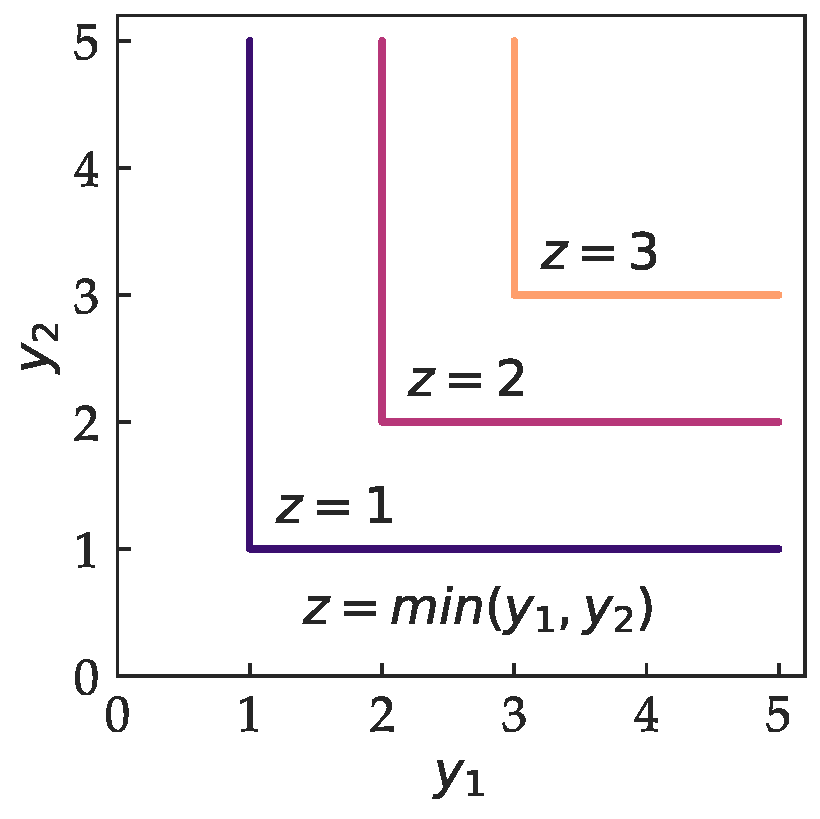
\includegraphics[width=\textwidth, height=\textwidth]{Figures/Essential.pdf}
    \end{minipage}
    \\ 
    %\begin{minipage}[t]{5cm}
    \vspace{-5pt}
    \uline{Interactive Essential:} In interactive essential interaction, we get diminishing return (instead of zero return) for a single factor: $z = y_1y_2$~\cite{tilman1980}. If factors are consumed using power basis function, i.e., $y_i = ax^\lambda_i$, it captures Cobb-Douglas production function.
    %\end{minipage} 
    &
    \begin{minipage}{.17\textwidth}
      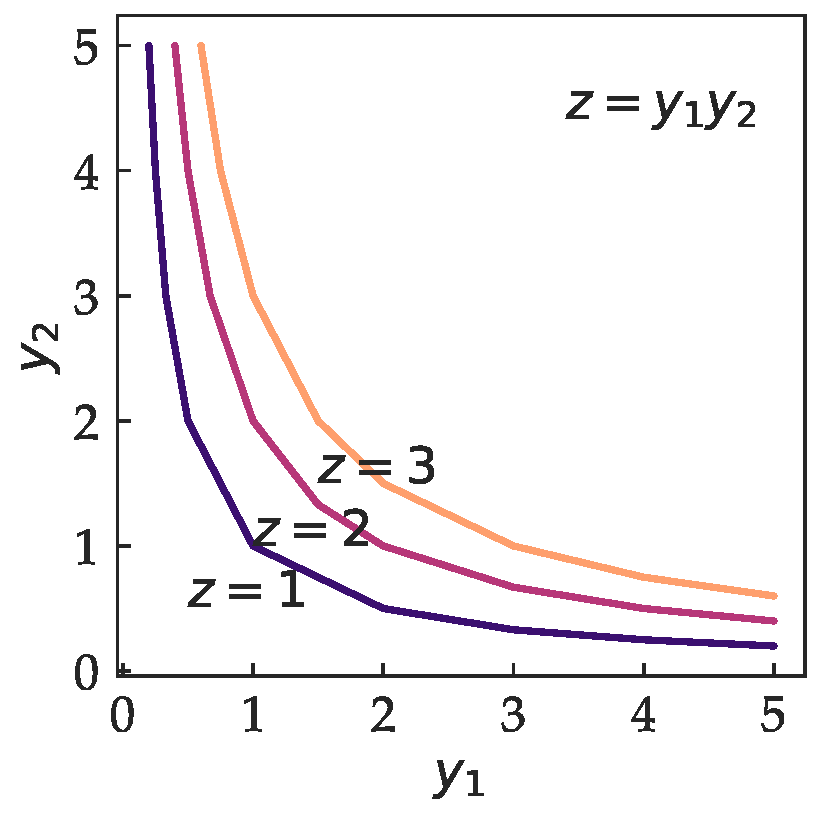
\includegraphics[width=\textwidth, height=.975\textwidth]{Figures/Interactive_Essential.pdf}
    \end{minipage}
    \\
    %\begin{minipage}[t]{5cm}
    \vspace{-5pt}
    \uline{Antagonistic:} For antagonistic factors, content generation is determined solely by the availability of the factor which yields the largest return: $z = max(y_1, y_2)$~\cite{tilman1980}. This interaction implies that the production process has maximum possible efficiency. 
    %\end{minipage} 
    &
    \begin{minipage}{.17\textwidth}
      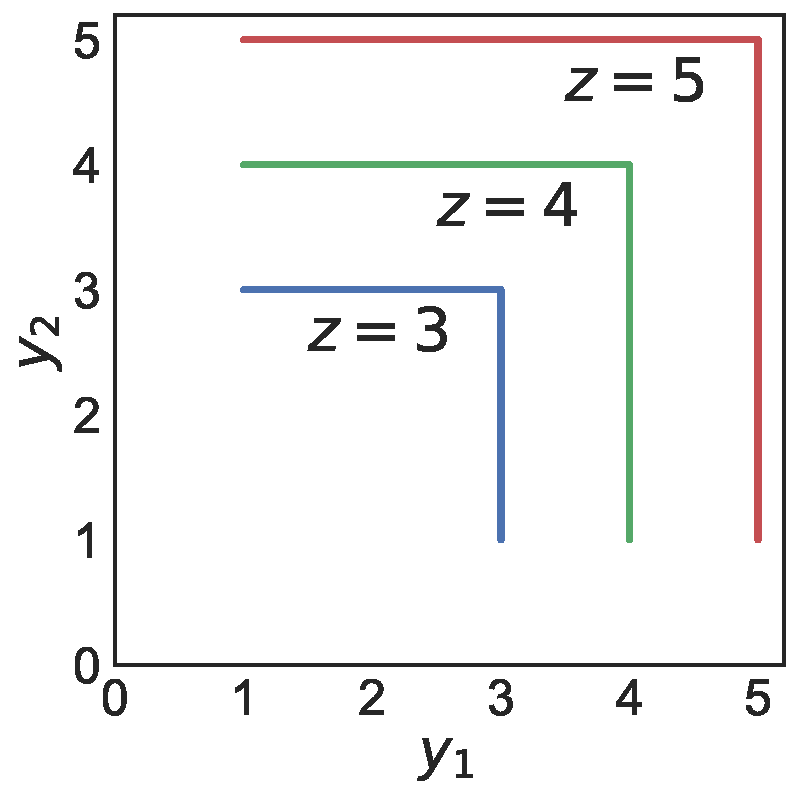
\includegraphics[width=\textwidth, height=.975\textwidth]{Figures/Antagonistic.pdf}
    \end{minipage}
    \\
    %\begin{minipage}[t]{5cm}
    \vspace{-5pt}
    \uline{Substitutable:} Factors that can each support production on their own are substitutable relative to each other: $z = w_1y_1 + w_2y_2$~\cite{tilman1980}. This implies that there exists some equivalence between the two factors. This is analogous to the general additive models.
    %\end{minipage} 
    &
    \begin{minipage}{.17\textwidth}
      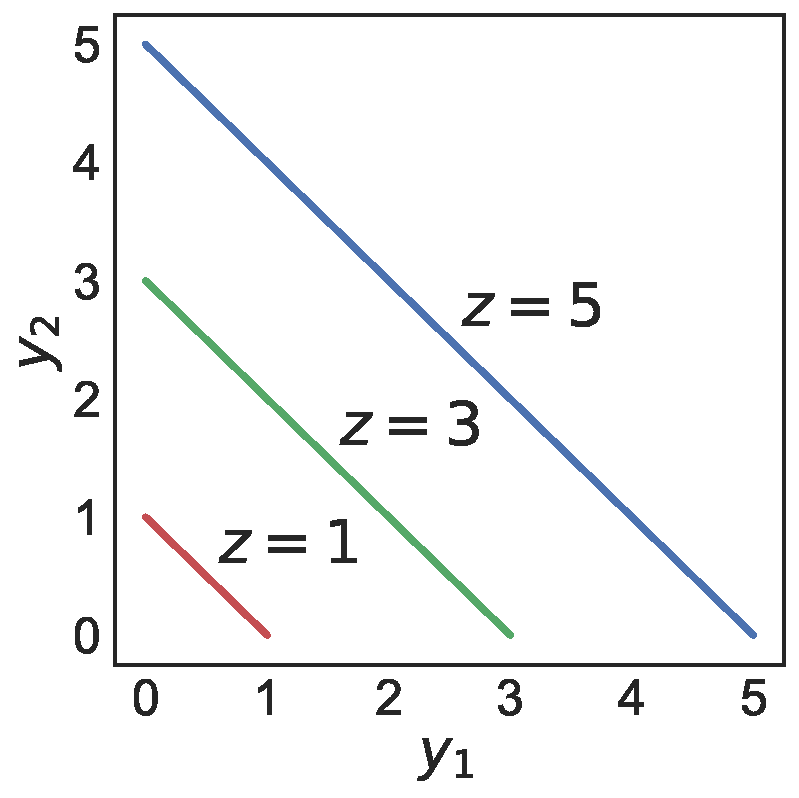
\includegraphics[width=\textwidth, height=.975\textwidth]{Figures/Substitutable.pdf}
    \end{minipage}
    \\
    \bottomrule
%    \hline
  \end{tabular}
  \vspace{-\baselineskip}
\end{table}

We combine basis function and interaction type to design production models for different content types. For example, answer generation can be modeled using power basis and essential interaction as $N_a = min(A_1N_q^{\lambda_1},A_2U_a^{\lambda_2})$. We consider twelve such possible models (combination of three basis and four interaction type) for answer and comment generation in Stack Exchange.

\textbf{User Role Distribution.} A fundamental assumption of our model is the awareness of user roles (e.g., asker, answerer, commenter) and their distribution (e.g., how many users are askers?). We empirically observe that all Stack Exchange markets have a stable distribution of user roles. In fact, given the number of users, we can accurately predict the number of participants of a particular role. In Figure~\ref{fig:roles} we show the distribution of $r^2$ for predicting user roles in Stack Exchange markets using linear regression. We observe that, in most markets, the number of participants of a role is a linear function of number of users.

\begin{figure}[hbt]
\vspace{-\baselineskip}
\centering
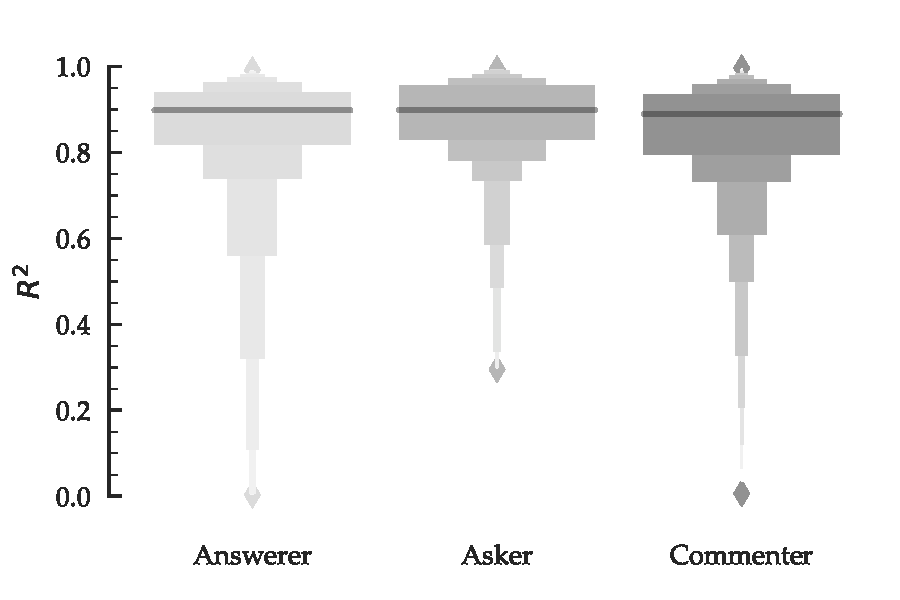
\includegraphics[scale=0.45]{Figures/User_to_Roles_R_Squared_LV.pdf}
\vspace{-\baselineskip}
\caption{The $r^2$ distribution for predicting user roles in Stack Exchange. In most Stack Exchange, the role distribution is stable---as manifested by the high median $r^2$ in letter value plots.}
\vspace{-\baselineskip}
\label{fig:roles}
\end{figure}

\textbf{Number of Users.} The number of users is the only free input to our content generation models; the remaining inputs are functions of number of users. In all these models, the growth or decline of number of users is exogenous---determined outside the model, by non-economic forces. There is a growing body of literature that concentrate on modeling active user growth~\cite{Ribeiro2014}. In this paper, we build upon these works to concentrate on a subsequent problem---the relation between user growth and content generation.



